\documentclass[a4paper]{article}

\usepackage[english]{babel}
\usepackage{amsmath}
\usepackage{graphicx}
%\usepackage{algorithm}
%\usepackage{algorithmic}
%\usepackage{algpseudocode}
\usepackage{url}


\title{Omega3P Integration Progress Report}

\author{Cameron W. Smith, Gerrett Diamond}

\date{\today}

\begin{document}
\maketitle

\section{In-memory Integration}



\section{Load Balancing}

Omega3P solving step relies on both on part mesh entities as well as a layer of 
ghosted elements along each part boundary. Figure \ref{fig:ghost3} shows an 
example of a mesh with three layers of ghosting. In order to reach maximum efficiency
for ghost based codes partitioning much target minimizing the sum of the 
weights of elements plus the sum of the weights of the ghost elements. 

\begin{figure}[ht]
\centering
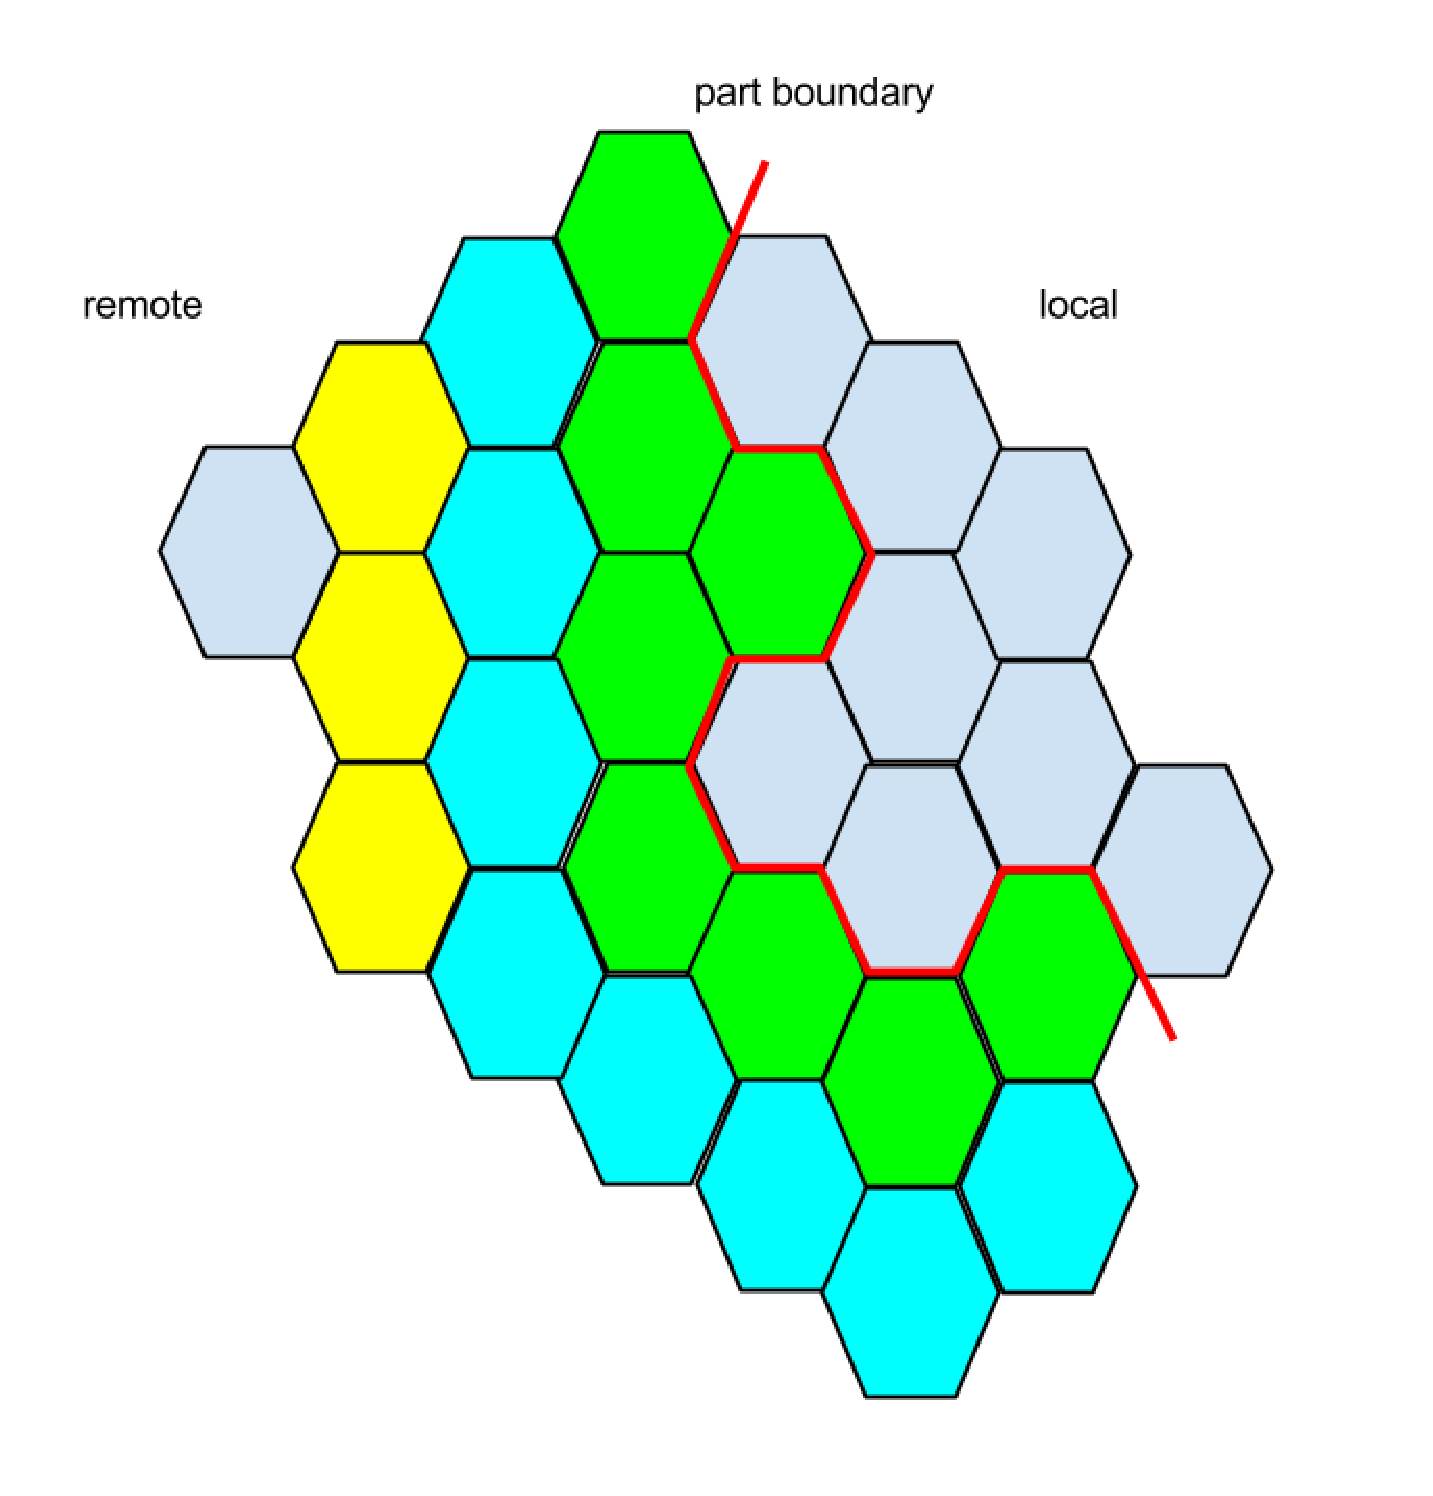
\includegraphics[width=0.3\textwidth]{ghostingExample.eps} 
\caption{\label{fig:ghost3} Three layers of elements ghosted from the remote part to the local part.  The first layer is colored green, the second blue, and the third yellow.}
\end{figure}

\noindent Our strategy for partitioning and load balancing is started with a 
uniformly-weighted 
partition of the mesh from 1 part to $N$ parts followed by ghost-aware diffusive load 
balancing using ParMA~\cite{SmithParma2015} to get a final mesh that is well balanced 
in terms of on-part elements and ghosted elements along the part's boundary. We 
currently utilize ParMA's partition improvement procedures that account for the 
ghosted layers using a combination of existing element selection criteria and an 
extended 'weight' tracking mechanism.  The weight tracking extension relies on the 
exact knowledge of the change to the ghosted elements as elements on a heavy part 
are selected for migration to a light part. The current implementation of these 
procedures assumes vertex-based ghosting while Omega3P ghosting is element-based. 
To accurately accommodate for Omega3P's ghosting we will be extending ParMA's 
ghosting to be able to balance based on element-based ghosting. To further improve 
the efficiency of the load balancing we may explore better partitionings 
that are ghost-aware so that ParMA is given a better initial partitioning such that it 
can find a better partitioning faster.

\section{Status}

\section{Results}


\newpage
\bibliographystyle{plain}
\bibliography{scorec-refs/partition,scorec-refs/meshdb}


\end{document}


